\chapter{자료 범위와 추가 검증}
\label{app:evidence_scope}
이 부록은 본문의 결론을 해석할 때 필요한 식별 조건, 서비스별 관측 범위, 대체 설명을 정리한다. 방향점수의 계산 안정성과 실제 비용부담의 인과적 식별은 서로 다른 검증 과제다.

\section{사건연구와 인과적 식별}

협의 사건 표본 \texttt{9/9}가 사전추세 검정을 통과하지 못했다. 표~\ref{tab:claim_placebo_event}와 그림~\ref{fig:claim_placebo_event}에서 웹툰 위약 사건(placebo)도 실제 사건(actual)과 비슷한 사전추세를 보인다. 특히 \texttt{treated\_rel\_m1}의 방향과 유의성이 유사하다. 이 표본의 사건계수는 정책이나 시장 사건의 인과효과로 해석할 수 없다.

\begin{table}[H]
\centering
\caption{위약 사건과 실제 사건의 추정결과 비교}
\label{tab:claim_placebo_event}
\small
\begin{tabular}{p{2.1cm}rrrl}
\toprule
\rowcolor{ReportTableHead}
상대 시점 & placebo 계수 & placebo p값 & actual 계수 & 해석 \\
\midrule
\texttt{m1} & -72.105 & 0.002 & -68.795 & 방향과 유의성이 거의 동일 \\
\texttt{p1} & 17.816 & 0.431 & 8.533 & 양측 모두 유의하지 않음 \\
\texttt{p2} & 24.330 & 0.419 & 10.884 & 양측 모두 유의하지 않음 \\
\bottomrule
\end{tabular}

\vspace{0.3em}
{\par\raggedright\footnotesize 주: 위약 사건과 실제 사건 모두 사전추세 판정은 \texttt{fail}이다. 사후 계수를 사건의 인과효과로 해석하기 위한 조건이 충족되지 않았다.\par}
\end{table}

\begin{figure}[H]
\centering
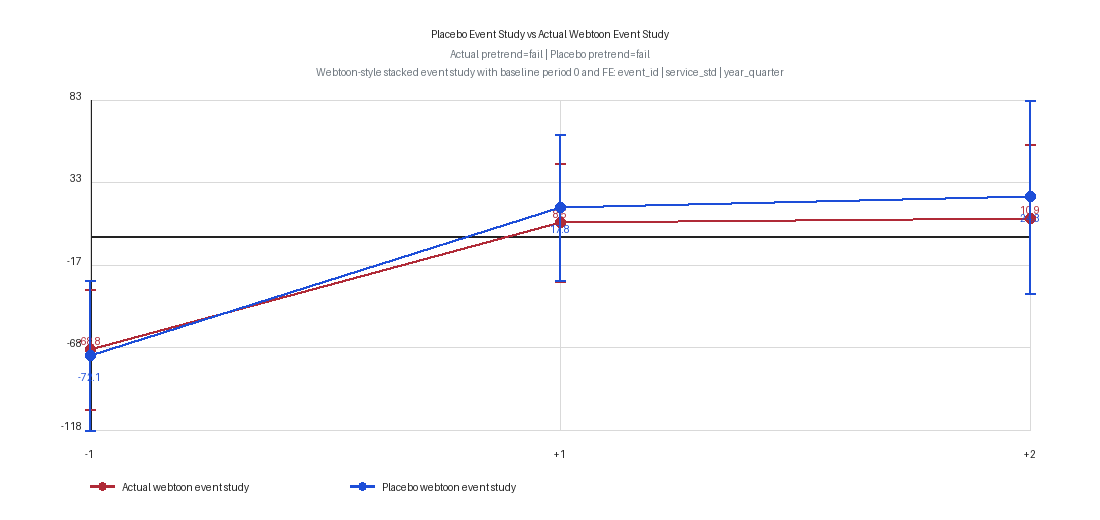
\includegraphics[width=0.88\textwidth]{outputs/figures/claim_strengthening/F_claim_placebo_event_plot.png}
\caption{위약 사건과 실제 사건의 사건연구 비교도}
\label{fig:claim_placebo_event}
\end{figure}

\section{비교사례의 관측 범위}
한국시장 확장 방향점수는 세 분야 모두 양수이고, 본문의 관측축 제외·가중치 변경에서도 그 방향이 유지된다. 별도로 적용한 엄격한 종합 판정기준은 자료의 직접성, 비교 가능성, 대체 설명까지 요구한다. 이 기준을 모두 충족한 직접 비교행은 0개였으며, 모든 분야에 일반화하는 강한 결론의 판정기준은 검토한 모든 시나리오에서 충족되지 않았다. 방향의 반복성이 확인되었다는 결과와 인과적 일반화에 필요한 자료가 더 있다는 판단은 이처럼 평가 대상이 다르다.

웹툰 및 스토리의 사례는 핵심축 관측이 적다. 또한 \nolinkurl{spotify@kr}, \nolinkurl{youtube_music@kr}, \nolinkurl{apple_music@kr}, \nolinkurl{netflix@kr}의 동일 서비스 직접 부담자료에는 결측 또는 범위값만 제시된 항목이 있다. 인프라의 위험-회수 축은 KT에서 양수, SK Telecom·LG Uplus에서 음수다. 따라서 정책은 종합점수와 함께 기업·채널별 부담을 확인해야 한다. 공식 요금 공시와 공정거래위원회의 유튜브 결합상품 시정자료는 해당 상품·집행 사실을 확인하는 별도의 근거다.

음악 확장 분석에서 공개자료로 확인한 항목과 추가 자료가 필요한 항목은 다음과 같다.

\begingroup
\footnotesize
\begin{summarylist}
  \item \textbf{라이선스 공개식 비중 격차}. 상태: 자료공개 여부의 코딩. 값: 1.000. 해석: 검토한 자료에서 국내 기준식과 해외 계약식의 공개범위가 다르다.
  \item \textbf{멜론 대 스포티파이 투명성 격차}. 상태: 투명성 항목의 연구 코딩. 값/경계: 4. 해석: 검토한 상품·계약자료의 공개범위 차이를 항목 수로 정리한 값이다.
  \item \textbf{멜론 대 유튜브 뮤직 투명성 격차}. 상태: 투명성 항목의 연구 코딩. 값/경계: 4. 해석: 유사 음원상품 비교의 자료공개 차이를 정리한 값이다.
  \item \textbf{법인 회계상 유효세율 차이}. 상태: 공시 추출값의 산술 비교. 값: 0.379(약 37.9\%p). 해석: FY2025 Dreamus와 Spotify 법인의 법인세비용/세전이익 차이다. 같은 회계연도의 비교이며, 한국 음악서비스의 현금세부담 귀착을 확인하려면 연결범위·이연법인세·서비스별 배분자료가 필요하다.
  \item \textbf{실제 해외 라이선스 요율 격차}. 상태: 미식별. 값/경계: --. 해석: 해외 계약 원문, 분모, 결합상품 범위 조정이 공개되지 않는다.
  \item \textbf{한국 대상 해외 상품 세부담 귀착 격차}. 상태: 미식별. 값/경계: --. 해석: 상품 단위 한국 세금 행과 법인-상품 배분 기준이 없다.
\end{summarylist}
{\par\raggedright\footnotesize 주: 투명성 격차는 공개범위를 연구 코딩규칙으로 정리한 값이다. 실제 해외 라이선스 요율과 한국 대상 상품의 세부담 귀착을 확인하려면 계약 및 서비스별 배분자료가 필요하다. 공개범위의 차이만으로 탈세 여부나 세금 회피 규모를 판정할 수 없다.\par}
\endgroup

\section{대체 설명과 후속 자료}
규모, 품질, 브랜드, 관측시점과 자료 가용성은 부담 차이에 영향을 줄 수 있다. 다음은 각 설명을 현재 분석에서 얼마나 줄였는지에 대한 점검 결과다. 잔여위험이 있다는 판정은 해당 요인이 관측된 차이의 일부를 설명할 가능성이 남아 있다는 뜻이다.

\begingroup
\small
\begin{summarylist}
  \item \textbf{단순 규모 차이}. 상태: 부분 축소. 잔여위험: 높음.
  \item \textbf{서비스 품질 차이}. 상태: 미해소. 잔여위험: 높음.
  \item \textbf{브랜드 및 네트워크 효과 차이}. 상태: 미해소. 잔여위험: 높음.
  \item \textbf{시기 차이}. 상태: 부분 축소. 잔여위험: 중간.
  \item \textbf{국가별 거시환경 차이}. 상태: 부분 축소. 잔여위험: 중간.
  \item \textbf{상장사·비상장사 공시 가용성 차이}. 상태: 미해소. 잔여위험: 높음.
  \item \textbf{제품 범위 차이}. 상태: 상당 축소. 잔여위험: 중간.
  \item \textbf{비교군 매칭 실패 또는 비교단위 불일치}. 상태: 부분 축소. 잔여위험: 중간.
  \item \textbf{proxy 및 측정오차 가설}. 상태: 미해소. 잔여위험: 높음.
\end{summarylist}
{\par\raggedright\footnotesize 주: 전체 분포는 \texttt{substantially\_reduced 1}, \texttt{partially\_reduced 4}, \texttt{still\_open 4}이며, \nolinkurl{can_still_weaken_claim=yes}는 \texttt{9/9}다.\par}
\endgroup

비공개 계약조건, 추천·노출 기준, 실시간 거래자료는 공개자료만으로 확인하기 어렵다. 후속 수집에서는 서비스별 비용·정산자료와 품질·전환·유지율 자료를 같은 시장·기간으로 맞추어, 이들 요인이 부담 차이를 얼마나 설명하는지 검증한다.

